% ============================================================
%  Nguyễn Trọng Đạt — CV (normalized, with a little personality)
%  Build:  xelatex cv.tex      Needs: figure/ folder next to this file
% ============================================================
\documentclass[10pt, a4paper]{article}

\usepackage{fontspec}
\setmainfont{Latin Modern Sans}   % clean sans; ships with every TeX Live
\setmonofont{Latin Modern Mono}   % used for the little "filename" captions

\usepackage[top=1cm, bottom=1cm, left=1.2cm, right=1.2cm]{geometry}
\usepackage[dvipsnames]{xcolor}
\usepackage{graphicx}
\usepackage{enumitem}
\usepackage{microtype}
\usepackage[most]{tcolorbox}
\usepackage[hidelinks]{hyperref}

\pagestyle{empty}
\setlength{\parindent}{0pt}
\setlength{\parskip}{0pt}
\raggedbottom

% Palette borrowed from your terminal theme
\definecolor{ink}{HTML}{2D3142}      % dark window background
\definecolor{slate}{HTML}{4F5D75}    % window border
\definecolor{accent}{HTML}{028090}   % teal
\definecolor{hi}{HTML}{1865FF}       % highlight blue
\definecolor{mint}{HTML}{35AE69}
\definecolor{muted}{HTML}{6B7280}
\definecolor{panel}{HTML}{EEF1F4}    % light sidebar panel
\definecolor{headtxt}{HTML}{C9D6E8}

\newcommand{\sep}{\;\textcolor{accent}{\textbullet}\;}
\newcommand{\mono}[1]{{\ttfamily\footnotesize #1}}

\setlist[itemize]{leftmargin=1.1em, itemsep=1.5pt, topsep=2pt, parsep=0pt,
                  label=\textcolor{accent}{\textbullet}}

% Section heading: teal bar + small caps text
\newcommand{\sect}[1]{\par\vspace{0.9em}%
  {\color{accent}\rule[-0.2ex]{3pt}{1.1em}}\hspace{5pt}{\large\bfseries\scshape\color{ink}#1}\par\vspace{0.4em}}

% Entry line: bold title + right info, italic subtitle + right info
\newcommand{\entry}[4]{%
  \textbf{#1}\hfill {\small\color{muted}#2}\\[-0.1em]
  {\small\itshape\color{accent}#3}\hfill {\small\itshape\color{muted}#4}\par\vspace{0.25em}}

% Framed screenshot with a monospace "filename" caption underneath
% \shot{width}{file}{caption}
\newcommand{\shot}[3]{%
  \begin{minipage}[t]{#1}\centering\vspace{0pt}
    \tcbox[enhanced, boxsep=0pt, left=0pt, right=0pt, top=0pt, bottom=0pt,
           arc=4pt, boxrule=0.8pt, colframe=slate, colback=white, clip upper,
           nobeforeafter]{\includegraphics[width=\dimexpr\linewidth-1.6pt\relax]{#2}}\\[-0.1em]
    {\color{muted}\mono{#3}}
  \end{minipage}}

\begin{document}

% ======================= PAGE 1 =======================

% ---------- Header banner ----------
\begin{tcolorbox}[enhanced, colback=ink, colframe=slate, arc=6pt, boxrule=1pt,
                  left=12pt, right=12pt, top=10pt, bottom=10pt, boxsep=0pt]
  \begin{minipage}[c]{0.74\linewidth}
    {\fontsize{26}{30}\selectfont\bfseries\color{white} Nguyễn Trọng Đạt}\\[0.5em]
    {\large\color{accent!45!white} Computer Engineering Student}\\[0.1em]
    {\color{headtxt} Robotics \sep AI \sep Drones \sep Embedded Systems}\\[0.9em]
    {\small\color{headtxt}
      Ho Chi Minh City, Vietnam \sep (+84) 399 922 395 \\[0.2em]
      \href{mailto:trongdat4work@gmail.com}{\color{headtxt}trongdat4work@gmail.com} \sep
      \href{https://github.com/LemonKronos}{\color{headtxt}github.com/LemonKronos} \sep
      \href{https://www.linkedin.com/in/trong-dat}{\color{headtxt}linkedin.com/in/trong-dat}}
  \end{minipage}\hfill
  \begin{minipage}[c]{0.2\linewidth}\raggedleft
    \tcbox[enhanced, boxsep=0pt, left=0pt, right=0pt, top=0pt, bottom=0pt,
           arc=6pt, boxrule=1pt, colframe=headtxt, clip upper, nobeforeafter]%
      {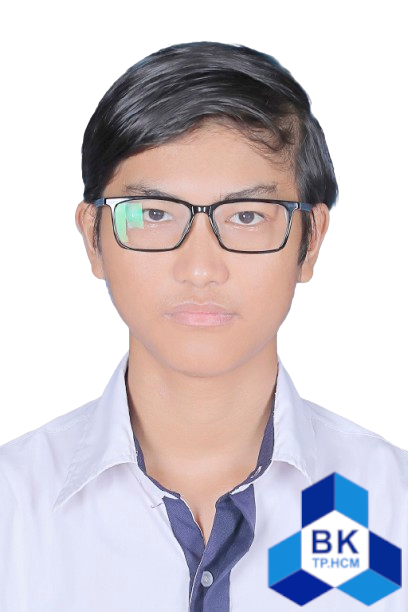
\includegraphics[height=3.6cm]{figure/MeFaceBK.png}}
  \end{minipage}
\end{tcolorbox}

\vspace{0.6em}

% ---------- Two columns ----------
\begin{minipage}[t]{0.30\linewidth}\vspace{0pt}
  \begin{tcolorbox}[enhanced, colback=panel, colframe=panel, arc=5pt,
                    left=8pt, right=8pt, top=2pt, bottom=8pt, boxsep=0pt]
    \sect{Education}
    \textbf{Ho Chi Minh University of Technology (HCMUT -- BKU)}\\[0.2em]
    B.Eng.\ in Computer Engineering\\
    {\small\color{muted}Expected graduation 2027}\\
    {\small\color{muted}GPA: 2.9/4.0}\\[0.4em]
    {\small\textbf{Coursework:} Embedded Systems, Operating Systems, Machine Learning,
    Microprocessors \& Microcontrollers, IoT-Oriented Logic Design, AI-Oriented Multidisciplinary Project}

    \sect{Skills}
    {\small
    \textbf{\color{accent}Programming}\\
    C++, Python, Rust\\
    {\color{muted}also C, Shell script;\\ familiar with Java, Go, Zig}\\[0.5em]
    \textbf{\color{accent}Robotics}\\
    ROS2 (Jazzy), Gazebo Harmonic, PX4 Autopilot, Micro XRCE-DDS\\[0.5em]
    \textbf{\color{accent}AI / ML}\\
    Reinforcement Learning, Imitation Learning, Latent Diffusion Learning, PyTorch,
    robotic data processing, AI edge computing\\[0.5em]
    \textbf{\color{accent}Tools}\\
    Git, Linux, VS Code}

    \sect{Languages}
    {\small
    \textbf{English} -- TOEIC L\&R 970/990\\
    \textbf{Vietnamese} -- native}

    \sect{Interests}
    {\small Drones, open source, and the Linux community. Long-term goal: Robotics Engineer.}
  \end{tcolorbox}
\end{minipage}%
\hfill
\begin{minipage}[t]{0.67\linewidth}
  \vspace{-0.4em}
  \sect{Summary}
  Computer Engineering student focused on robotics, embedded systems, and autonomous drone software.
  Experienced with \textcolor{hi}{\textbf{ROS2, PX4, Gazebo, and C++}} for real-time systems and simulation,
  and comfortable contributing safely to shared Git codebases. Seeking a part-time engineering role, with the
  option of moving to full-time after graduation.

  \sect{Experience}
  \entry{Internship: Cross-Platform ITAM Endpoint Device Agent}{16/7 - 17/9/2026}{GSOFT SOFTWARE}{Ho Chi Minh City}
  \begin{itemize}
    \item Built a lightweight, memory-safe IT-asset monitoring daemon for Linux and Windows in
          \textbf{Rust} (Tokio, Unix domain sockets).
    \item Split the agent into separate binaries (launcher, worker, fetcher) connected by IPC, so a fetcher
          crash cannot take down the main daemon; scheduled tasks with a custom min-heap scheduler.
    \item Implemented OS-specific system calls and the IPC layer; profiled memory and CPU bottlenecks with
          flamegraph and hyperfine.
    \item Delivered a working cross-platform MVP with scheduled data fetching and resilient inter-process
          communication, with no memory leaks observed.
  \end{itemize}

  \sect{Featured Project}
  \textbf{Drone Simulation Pipeline} \hfill {\small\color{muted}Passion project}\\[0.2em]
  Built a ROS2 + PX4 + Gazebo simulation pipeline to train AI models for VTOL acrobatic flight (details on page 2).\\[0.5em]
  \shot{\linewidth}{figure/DemoDrone.png}{Drone\_Simulation\_Preview.png}
\end{minipage}

\newpage

% ======================= PAGE 2 =======================

% ---------- Project 1 ----------
\begin{tcolorbox}[enhanced, colback=white, colframe=slate, arc=6pt, boxrule=1pt,
                  left=10pt, right=10pt, top=6pt, bottom=8pt, boxsep=0pt,
                  colbacktitle=ink, coltitle=white, fonttitle=\bfseries,
                  title={Project 1 \quad Acrobatic Drone Pipeline with Latent Imitation Learning},
                  toptitle=3pt, bottomtitle=3pt]
  \entry{AI-Oriented Multidisciplinary Project}{2025}{ROS2, PX4, Gazebo Harmonic, Micro XRCE-DDS, Python}{}
  \begin{minipage}[t]{0.66\linewidth}\vspace{0pt}
    \begin{itemize}
      \item Built a simulation and control pipeline for an ``AI co-pilot'' that learns from expert pilot input
            and turns noisy human commands into safe 3D trajectories.
      \item Integrated Gazebo Harmonic (physics), PX4 (flight control, 400\,Hz), Micro XRCE-DDS (PX4--ROS2 link)
            and ROS2 (offboard middleware, 80\,Hz); the AI runs as a Python ROS2 node at 0.5\,Hz behind a safety
            and obstacle-avoidance layer.
      \item Collected expert control and telemetry data in a procedurally generated obstacle-tunnel world, trained
            models offline, and evaluated them offline and in real-time user-controlled flights.
      \item Validated the non-AI pipeline with autonomous flights of up to 1\,km without collisions (average
            simulated latency 290\,µs). Early AI-controlled results were noisy and sometimes conflicted with
            pilot input, which pointed to design and data-flow issues between the high- and low-level layers.
      \item Now redesigning the pipeline around low-level data processing, system integration and control
            structure to support more dynamic maneuvers.
    \end{itemize}
  \end{minipage}\hfill
  \begin{minipage}[t]{0.3\linewidth}\centering\vspace{0pt}
    \shot{5.0cm}{figure/OverviewPipeline.png}{System\_Pipeline.png}
  \end{minipage}

  \vspace{0.6em}
  \shot{0.485\linewidth}{figure/DemoDrone2.png}{Test\_non-AI\_behavior.png}\hfill
  \shot{0.485\linewidth}{figure/test_control_world.png}{Test\_Control\_World.png}
\end{tcolorbox}

\vspace{0.8em}

% ---------- Project 2 ----------
\begin{tcolorbox}[enhanced, colback=white, colframe=slate, arc=6pt, boxrule=1pt,
                  left=10pt, right=10pt, top=6pt, bottom=8pt, boxsep=0pt,
                  colbacktitle=ink, coltitle=white, fonttitle=\bfseries,
                  title={Project 2 \quad VTOL Acrobatic Flight \& Obstacle Avoidance with RL},
                  toptitle=3pt, bottomtitle=3pt]
  \entry{Capstone Project (in progress)}{2026}{C++, ROS2 Jazzy, PyTorch, Voxblox (ESDF), Gazebo Harmonic, PX4}{}
  \begin{minipage}[t]{0.6\linewidth}\vspace{0pt}
    \begin{itemize}
      \item Designing a pilot-intent-driven control architecture that gives pilots of any skill level expert-level
            control of a VTOL while keeping deterministic spatial safety.
      \item The policy takes pilot or planner intent, PX4-estimated drone state, and a 3D-CNN latent encoding of
            the Voxblox ESDF map, and outputs normalized actuator commands to the PX4 mixer.
      \item Staged RL curriculum (hover $\rightarrow$ tracking $\rightarrow$ obstacle avoidance), each stage with its own
            reward and an entropy objective to explore the flight envelope.
      \item Deterministic reactive fallback using APF path planning for extra safety.
    \end{itemize}
  \end{minipage}\hfill
  \begin{minipage}[t]{0.36\linewidth}\raggedleft\vspace{0pt}
    \shot{1.97cm}{figure/AlphaMinus1_cut.png}{VTOL.png}\hspace{4pt}%
    \shot{4.05cm}{figure/SpatialCNN.png}{3D CNN design.png}
  \end{minipage}
\end{tcolorbox}

\end{document}
